\documentclass{beamer}
\usepackage[utf8]{inputenc}
\usepackage[spanish]{babel}
\usepackage{hyperref}
\usepackage{verbatim}
\usepackage{listings}

\setbeamercovered{invisible}
\usetheme{Frankfurt}
\usefonttheme{serif}

% Configurar los listings (Códigos)
\renewcommand{\lstlistingname}{Código}
\lstset{
	language=C++,               % Lenguaje
	basicstyle=\ttfamily\footnotesize,  % Tipo de fuente
	keywordstyle=\color{blue},  % Color de palabras clave
	stringstyle=\color{red},    % Color de strings
	commentstyle=\color{gray},  % Color de comentarios
	showstringspaces=false,     % No muestrar el _ cuando el string tiene espacios
	breaklines = true,          % Partir las líneas largas
	breakatwhitespace=true,	    % Partir las líneas en un espacio
	numbers=left,				% Numerar las líneas a la izq
	numberstyle=\tiny,			% Poner los números de las líneas pequeños
	numberblanklines=true,      % Numerar las líneas en blanco
	columns=fullflexible,       % No perder el formato al dejar los espacios
	keepspaces=true,   			% Dejar los espacios insertados
	frame=tb,					% Poner el recuadro
}


\title{Semillero de Programación}
\subtitle{Problemas con DFS, BFS, Componentes Fuertemente Conexas y Ordenamiento Topológico}
\author{Ana Echavarría \and Juan Francisco Cardona}

\institute{Universidad EAFIT}
\date{1 de marzo de 2013}

\begin{document}

\begin{frame}
	\titlepage
\end{frame}

\begin{frame}
	\frametitle{Contenido}
	\tableofcontents
\end{frame}

\section{Bicoloring}
	\begin{frame}
		\frametitle{Problema 10004 - Bicoloring}
		\begin{block}{Problema}
			Verificar si un grafo es bipartito, es decir, si se pueden usar dos colores para pintar todos los nodos de manera que dos nodos vecinos no tengan el mismo color
		\end{block}
	\end{frame}
	
	\begin{frame}
		\frametitle{¿Qué técnica usar?}
		\begin{alertblock}{Pregunta}
				\begin{itemize}
					\item ¿Cómo hago para verificar que el grafo sea bipartito? \pause
						\begin{itemize}
							\item Pinto el primer nodo de un color y todos sus vecinos de otro color y repito el proceso con los vecinos. \pause
						\end{itemize}
					\item ¿Qué pasa si tengo que pintar un nodo que ya pinté antes? \pause
						\begin{itemize}
							\item Si el color con el que lo tengo que pintar es el mismo que tiene no pasa nada, si no es así el grafo no es bipartito.
						\end{itemize}
					\item ¿Qué técnica puedo usar para pintar cada nodo y luego sus vecinos? \pause
						\begin{itemize}
							\item Se pueden usar BFS y DFS.
						\end{itemize}
				\end{itemize}
		\end{alertblock}
	\end{frame}
	
	\begin{frame}[fragile]
		\frametitle{Solución}
		\begin{lstlisting}
			int main(){
			   int n, m;
			   while (cin >> n){
			      if (n == 0) break;
			      for (int i = 0; i < n; ++i){
			         g[i].clear();
			         color[i] = -1;
			      }
			      cin >> m;
			      for (int i = 0; i < m; ++i){
			         int u, v;
			         cin >> u >> v;
			         g[u].push_back(v);
			         g[v].push_back(u);
			      }
			      if (dfs(0, 0)) puts("BICOLORABLE.");
			      else puts("NOT BICOLORABLE.");
			   }
			    return 0;
			}
		\end{lstlisting}
	\end{frame}
	
	\begin{frame}[fragile]
		\frametitle{Solución usando DFS}
		\begin{lstlisting}
			const int MAXN = 205;
			vector <int> g[MAXN];
			int color[MAXN];

			bool dfs(int u, int paint){
			   color[u] = paint;
			   for (int i = 0; i < g[u].size(); ++i){
			      int v = g[u][i];
			      bool possible;
			      if (color[v] == -1) possible = dfs(v, 1 - paint);
			      else possible = (color[v] == (1 - paint));
			      if (!possible) return false;
			   }
			   return true;
			}
		\end{lstlisting}
	\end{frame}
	
	\begin{frame}[fragile]
		\frametitle{Solución usando BFS}
		\begin{lstlisting}
		bool bfs(int s){
		   queue <int> q;
		   q.push(s);
		   color[s] = 0;
		   while (q.size() > 0){
		      int u = q.front(); q.pop();
		      for (int i = 0; i < g[u].size(); ++i){
		         int v = g[u][i];
		         if (color[v] == color[u]) return false;

		         if (color[v] == -1){
		            color[v] = 1 - color[u];
		            q.push(v);
		         }
		      }
		   }
		   return true;
		}
		\end{lstlisting}
	\end{frame}
	

\section{Playing with Wheels}
	\begin{frame}
		\frametitle{Problema 10067 - Playing with Wheels}
		Se tiene una caja fuerte con 4 ruedas que indican cada una un número. Cada rueda tiene dos botones, uno mueve la rueda a la derecha (aumenta el número mostrado y si es 9 cambia al 0) y el otro mueve la rueda a la izquierda (disminuye el número mostrado y si es 0 cambia al 9).
		\begin{center} 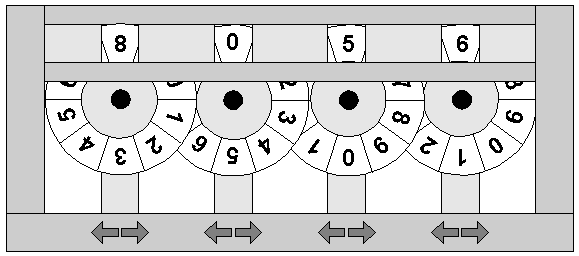
\includegraphics[height = 0.4\textheight]{wheels.png} \end{center}
	\end{frame}
	
	\begin{frame}
		\frametitle{Problema}
		\begin{itemize}
			\item Se sabe cuál es la configuración inicial de las ruedas y cuál es la configuración final que abre la caja fuerte. Sin embargo, hay un conjunto de configuraciones prohibidas que no se pueden activar.\\
			\item El problema es hallar el \textbf{mínimo número de movimientos de las ruedas que hay que hacer para llegar de la configuración inicial a la final sin pasar por ninguna de las configuraciones prohibidas.}
		\end{itemize}
	\end{frame}
	
	\begin{frame}
		\frametitle{¿Qué técnica usar?}
		\begin{alertblock}{Preguntas}
			\begin{enumerate}
				\item ¿El problema se puede expresar como un problema de grafos? \pause
				\item ¿Cuáles serían los nodos? \pause
				\item ¿Cuándo se forma una arista? (¿cuándo se unen dos nodos?) \pause
				\item ¿Cuántos nodos hay? \pause
				\item ¿Cuántas aristas hay? \pause
				\item ¿El grafo cambia con cada caso de prueba o es independiente de los casos de prueba? \pause
				\item ¿Cómo hallo el mínimo número de movimientos para llegar de un nodo al otro?
			\end{enumerate}
		\end{alertblock}
	\end{frame}
	
	\begin{frame}
		\frametitle{Representación del grafo}
		Cada nodo del grafo es un vector enteros de 4 posiciones, sin embargo en el algoritmo asumimos que los nodos son número enteros. ¿Hay alguna forma de representar estos nodos como números? ¿Si la hay, pueden dos nodos tener la misma representación?
	\end{frame}
	
	\begin{frame}[fragile]
		\frametitle{Creación del grafo}
		\begin{lstlisting}
			const int MAXN = 10005;
			// Find neighbour of node u if you move wheel d in direction dir
			int find_neighbour(int u, int d, int dir){
			   vector <int> a(4);
			   for (int i = 0; i < 4; ++i){
			      a[i] = u % 10;
			      u /= 10;
			   }
			   a[d] = (a[d] + 10 + dir) % 10;

			   int ans = 0;
			   for (int i = 3; i >= 0; --i){
			      ans *= 10; ans += a[i];
			   }
			   return ans;
			}
		\end{lstlisting}
	\end{frame}
	
	\begin{frame}[fragile]
		\frametitle{Creación del grafo y lectura números}
		\begin{lstlisting}
			vector <int> g[MAXN];
			void make_graph(){ // Create out edges for all nodes
			   for (int i = 0; i <= 9999; ++i){
			      for (int d = 0; d < 4; ++d){
			         g[i].push_back(find_neighbour(i, d, -1)); // Move left
			         g[i].push_back(find_neighbour(i, d, +1)); // Move right
			      }
			   }
			}
		\end{lstlisting}
		
		\begin{lstlisting}
			int get_num(){ // Read nodes and convert them to an integer
			   int ans = 0;
			   for (int i = 0; i < 4; ++i){
			      int d; cin >> d;
			      ans = ans * 10 + d;
			   }
			   return ans;
			}
		\end{lstlisting}
	\end{frame}
	
	\begin{frame}[fragile]
		\frametitle{Lectura de los datos}
		\begin{lstlisting}
			bool forbidden[MAXN]; // The forbidden edges
			int d[MAXN];            // The distance for start vertex

			int main(){
			   make_graph();        // Create the graph
			   int cases; cin >> cases;
			   while (cases--){
			      for (int i = 0; i < MAXN; ++i) forbidden[i] = false;
			      int s = get_num(); // Read start vertex
			      int t = get_num(); // Read end vertex

			      int n; cin >> n;   // Read all forbidden vertices
			      while (n--) forbidden[get_num()] = true;
		
			      bfs(s);               // Call bfs from the start vertex
			      cout << d[t] << endl; // Output distance to end vertex
			   }
			   return 0;
			}
		\end{lstlisting}
	\end{frame}
	
	\begin{frame}[fragile]
		\frametitle{BFS}
		\huge{Tarea}
		% \begin{lstlisting}
		% 			void bfs(int s){
		% 			   for (int i = 0; i < MAXN; ++i) d[i] = -1;
		% 			   queue <int> q;
		% 			   q.push(s);
		% 			   d[s] = 0;
		% 			   while (q.size() > 0){
		% 			      int cur = q.front(); q.pop();
		% 			      for (int i = 0; i < g[cur].size(); ++i){
		% 			         int next = g[cur][i];
		% 			         // If not seen before and not forbidden add to queue
		% 			         if (!forbidden[next] and d[next] == -1){ 
		% 			            d[next] = d[cur] + 1;
		% 			            q.push(next);
		% 			         }
		% 			      }
		% 			   }
		% 			}
		% 		\end{lstlisting}
	\end{frame}
\end{document}